\clearpage
\VerdierPhysicalPageAnchor{0237}%
\begingroup\small\setlength{\parskip}{0pt}\setlength{\emergencystretch}{1.5em}
\setlength{\abovedisplayskip}{4pt plus 2pt minus 2pt}%
\setlength{\belowdisplayskip}{4pt plus 2pt minus 2pt}%

\VerdierSemanticAnchor{ch4d-4-3-2}
\noindent\textbf{Proposition 4.3.2.}\quad
\textit{Let $X$ be an object of $\operatorname{comp}(\mathcal A)$, let
$\bigl(X(p,q),\delta(p,q,r)\bigr)$ be the second spectral object associated
with $X$, and let $H\colon D(\mathcal A)\longrightarrow\mathcal A$ be the
canonical cohomological functor.}

\VerdierSemanticAnchor{ch4d-4-3-2-a}
\noindent\textit{a) $H^r\bigl(X(p,q)\bigr)=0$ for every integer $r<p$ or
$r\geq q$.}

\VerdierSemanticAnchor{ch4d-4-3-2-b}
\noindent\textit{b) Let $r$ be an integer. For every element $(p,q)$ of
$\mathcal{F}\ell_1(\widetilde{\mathbb Z})$ such that $p\leq r<q$, there
exists a unique isomorphism}
\[
i_{p,q}^r(X)\colon H^r(X)\xrightarrow{\sim}H^r\bigl(X(p,q)\bigr)
\]
\noindent\textit{such that $i_{-\infty,+\infty}^r(X)$ is the identity and
such that, for every pair $(p,q)$ and $(p',q')$ with $p\leq p'$,
$q\leq q'$, $p\leq r<q$, and $p'\leq r<q'$, the following diagram is
commutative:}

\VerdierSemanticAnchor{ch4d-4-3-2-b-diagram}
\begin{center}
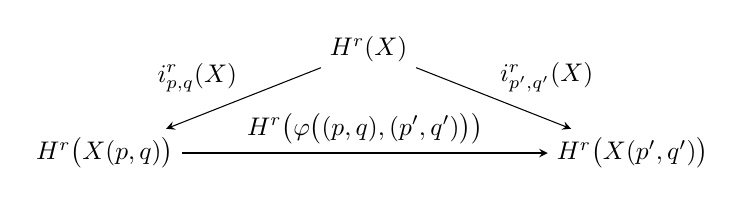
\begin{tikzpicture}[>=stealth,line width=.38pt,x=2.35cm,y=1.15cm,
  scale=.92,transform shape]
  \node (HX)  at (1.55,1.25) {$H^r(X)$};
  \node (Hpq) at (0,0) {$H^r\bigl(X(p,q)\bigr)$};
  \node (Hpp) at (3.10,0) {$H^r\bigl(X(p',q')\bigr)$};
  \draw[->] (HX) -- node[above left=-1pt] {$i_{p,q}^r(X)$} (Hpq);
  \draw[->] (HX) -- node[above right=-1pt] {$i_{p',q'}^r(X)$} (Hpp);
  \draw[->] (Hpq) -- node[above]
    {$H^r\!\left(\varphi\bigl((p,q),(p',q')\bigr)\right)$} (Hpp);
\end{tikzpicture}
\end{center}

\VerdierSemanticAnchor{ch4d-4-3-2-c}
\noindent\textit{c) Let $m\colon X\longrightarrow Y$ be a morphism in
$\operatorname{comp}(\mathcal A)$, and let}
\[
m(p,q)\colon X(p,q)\longrightarrow Y(p,q)
\]
\noindent\textit{be the corresponding morphism between the associated
second spectral objects. For every element $(p,q)$ of
$\mathcal{F}\ell_1(\widetilde{\mathbb Z})$ and every integer $r$ such that
$p\leq r<q$, the following diagram is commutative:}

\VerdierSemanticAnchor{ch4d-4-3-2-c-diagram}
\begin{center}
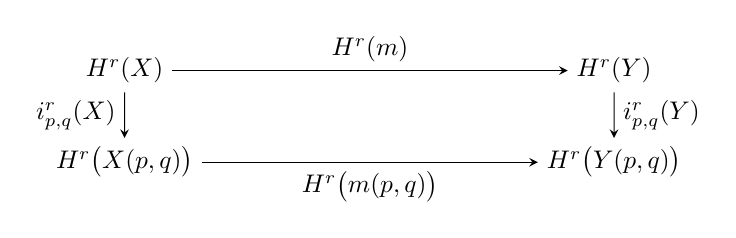
\begin{tikzpicture}[>=stealth,line width=.38pt,x=2.55cm,y=1.10cm,
  scale=.92,transform shape]
  \node (HX)  at (0,1.15) {$H^r(X)$};
  \node (HY)  at (2.65,1.15) {$H^r(Y)$};
  \node (Hpq) at (0,0) {$H^r\bigl(X(p,q)\bigr)$};
  \node (HpY) at (2.65,0) {$H^r\bigl(Y(p,q)\bigr)$};
  \draw[->] (HX) -- node[above] {$H^r(m)$} (HY);
  \draw[->] (Hpq) -- node[below] {$H^r\bigl(m(p,q)\bigr)$} (HpY);
  \draw[->] (HX) -- node[left] {$i_{p,q}^r(X)$} (Hpq);
  \draw[->] (HY) -- node[right] {$i_{p,q}^r(Y)$} (HpY);
\end{tikzpicture}
\end{center}

\noindent This proposition follows immediately from the definitions.

\VerdierSemanticAnchor{ch4d-4-3-3}
\medskip\noindent\textbf{Corollary 4.3.3.}\quad
\textit{The second canonical spectral-object functor (4.3.1) factors
uniquely through the canonical functor}
\[
\operatorname{comp}(\mathcal A)\longrightarrow D(\mathcal A).
\]

\VerdierSemanticAnchor{ch4d-4-3-3-proof}
Indeed, by (4.3.2), this functor takes a quasi-isomorphism
$m\colon X\longrightarrow Y$ to an isomorphism of spectral objects. The
corollary therefore follows from (1.3.5).
\endgroup
